\documentclass[a4paper, 12pt]{article}

\usepackage[T2A]{fontenc}
\usepackage[utf8]{inputenc}
\usepackage[english,russian]{babel}
\usepackage[left=15mm, top=20mm, right=15mm, bottom=20mm, nohead, nofoot]{geometry}

\usepackage{hyperref}
\usepackage{graphicx}
\usepackage{wrapfig}
\usepackage{afterpage}
\usepackage{amsmath, amsfonts, amssymb, amsthm, mathtools}
\author{Хомутов Андрей, группа Б06-903}
\title{ВПВ по курсу "Электричество и магнетизм" \\ Конденсатор на высоких частотах}
\date{22 декабря 2020 г.}
%%%%%%%%%%%%%%%%%%%%%%%%%%%%%%%%%%%%%%%%%%%%%%%%%%%%%%%%%%%%%%%%%%%%%%%%%
\usepackage{graphicx, wrapfig, subcaption, setspace, booktabs}
\usepackage[protrusion=true, expansion=true]{microtype}
\usepackage[english]{babel}
\usepackage{sectsty}
\usepackage{url, lipsum}
\newcommand{\HRule}[1]{\rule{\linewidth}{#1}}
\onehalfspacing
\setcounter{tocdepth}{5}
\setcounter{secnumdepth}{5}
%%%%%%%%%%%%%%%%%%%%%%%%%%%%%%%%%%%%%%%%%%%%%%%%%%%%%%%%%%%%%%%%%%%%%%%%%


\begin{document}

\title{ \normalsize \textsc{Лабораторная работа}
		\\ [4.0cm]
		\HRule{0.5pt} \\ [0.3cm]
		\LARGE \textbf{{Дифракция}}
		\HRule{0.5pt} \\ [0.1cm]
		\normalsize  \vspace*{18\baselineskip}}

\date{}

\author{%Шамарина Екатерина, Б06-903 \\
		Хомутов Андрей, Б06-903 \\
ФБМФ, 2021\\ }

\maketitle
\thispagestyle{empty}
\newpage
%%%%%%%%%%%%%%%%%%%%%%%%%%%%%%%%%%%%%%%%%%%%%%%%%%%%%%%%%%%%%%%%%%%%%%%%%
\section{Дифракция Френеля на щели}
	
\subsection{Экспериментальная установка}
	
	Схема установки для наблюдения дифракции Френеля на щели
представлена на рис. 1. Световые лучи освещают щель $ S_2 $ и испытывают на ней дифракцию. Дифракционная картина рассматривается с помощью микроскопа М, сфокусированного на некоторую плоскость наблюдения П.
	
	\begin{figure}[h!]
		\centering
		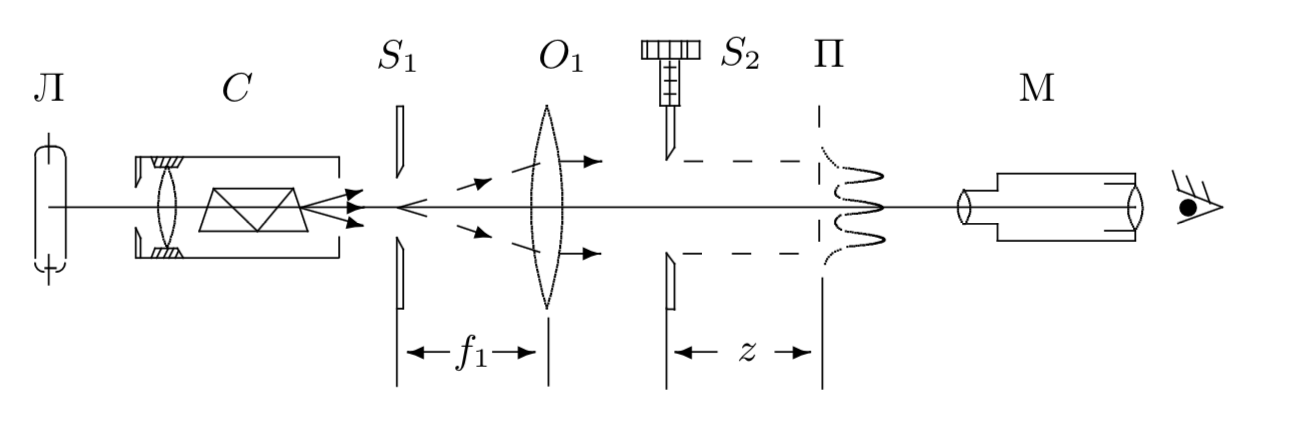
\includegraphics[width=0.8\linewidth]{a.png}
		\caption{Схема установки для наблюдения дифракции Френеля}
		\label{labA}
	\end{figure}

Щель $ S_2 $ освещается параллельным пучком монохроматического
света с помощью коллиматора, образованного объективом $ O_1 $, и щелью S1, находящейся в его фокусе. На щель $ S_1 $ сфокусировано изображение спектральной линии, выделенной из спектра ртутной лампы Л при помощи простого монохроматора C, в котором используется приз-
ма прямого зрения.

Распределение интенсивности света в плоскости наблюдения П про-
ще всего рассчитывать с помощью зон Френеля (для щели их иногда
называют зонами Шустера). При освещении щели $ S_2 $ параллельным пучком лучей (плоская волна) зоны Френеля представляют собой по-
лоски, параллельные краям щели (рис. 2). Результирующая амплитуда
в точке наблюдения определяется суперпозицией колебаний от тех зон
Френеля, которые не перекрыты створками щели. Графическое определение результирующей амплитуды производится с помощью векторной
диаграммы --- спирали Корню. Суммарная ширина $ n $ зон Френеля (Шустера) определяется соотношением:
\begin{equation}\label{xin}
\xi_n = \sqrt{zn\lambda}
\end{equation}
где $ z $ --- расстояние от щели до плоскости наблюдения (рис. 1), а $ \lambda $ --- длина волны.

\begin{wrapfigure}{r}{0.25\linewidth} 
	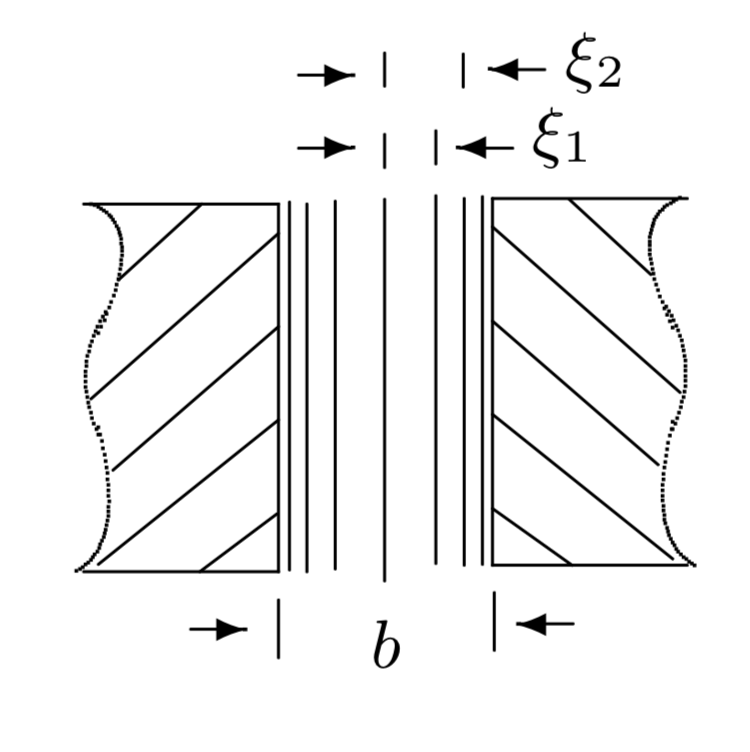
\includegraphics[width=\linewidth]{zone}
	\caption{Зоны Френеля}
	\label{zone}
\end{wrapfigure}

Вид наблюдаемой дифракционной картины
на щели шириной $ b $ определяется волновым параметром $ p $ или числом Френеля $ C $ (число открытых полных зон):


$$
p = \dfrac{\sqrt{z \lambda}}{b}, \qquad C = \dfrac{1}{p^2}.
$$

Дифракционная картина отсутствует вблизи щели при $ p \ll 1 $
($ C \gg 1 $, т. е. на щели укладывается огромное число зон), а распределение интенсивности света за щелью можно приближённо получить
с помощью законов геометрической оптики. Дифракционная картина
в этом случае наблюдается только в узкой области на границе света и
тени у краёв экрана.

При небольшом удалении от щели (или изменении ширины щели $ S_2 $) эти две группы дифракционных полос перемещаются практически независимо друг от друга. Каждая из этих групп образует картину дифракции Френеля на краю экрана. Распределение интенсивности
при дифракции света на краю экрана может быть найдено с помощью
спирали Корню.

При дальнейшем увеличении расстояния $ z $ (или уменьшении шири-
ны щели $ S_2 $) обе системы дифракционных полос постепенно сближаются и, наконец, при $ C \gtrsim 1 $ накладываются друг на друга. Распределение интенсивности в плоскости наблюдения в этом случае определяется
числом зон Френеля, укладывающихся на полуширине щели $ b/2 $. Если это число равно $ n $, то в поле зрения наблюдается $ m = n - 1 $ тёмных полос. Таким образом, по виду дифракционной картины можно оценить
число зон Френеля на полуширине щели.

\subsection{Практическая часть}

Ширина щели - $D_0 = 0.28 \pm 0.1$ мм. В таблице 1 записаны координаты микроскопа в зависимости от количества полос на экране. Вычтя из них координату щели $x_0 =$ 50.2 см, получим z - координату по рисунку 1. Рассчитав по формуле (1) $D= 2\xi_n $ сравним полученую величину с $D_0$ на рис. 2. Для зеленой линии ртути $\lambda = $ 546.1 нм.

\begin{table}[h!]
\begin{center}
\caption{Эксперимент с дифракцией Френеля}
\begin{tabular}{|c|c|c|c|c|}
\hline
Количество полос & х, см & z, см & D, mm & $\delta_D$, mm \\ \hline
1                & 53,2  & 3     & 0,26  & 0,02           \\ \hline
2                & 51,8  & 1,6   & 0,26  & 0,03           \\ \hline
3                & 51,5  & 1,3   & 0,29  & 0,04           \\ \hline
4                & 51,1  & 0,9   & 0,28  & 0,06           \\ \hline
5                & 51    & 0,8   & 0,30  & 0,07           \\ \hline
\end{tabular}
\end{center}
\end{table}

\begin{figure}[h!]
    \begin{center}
    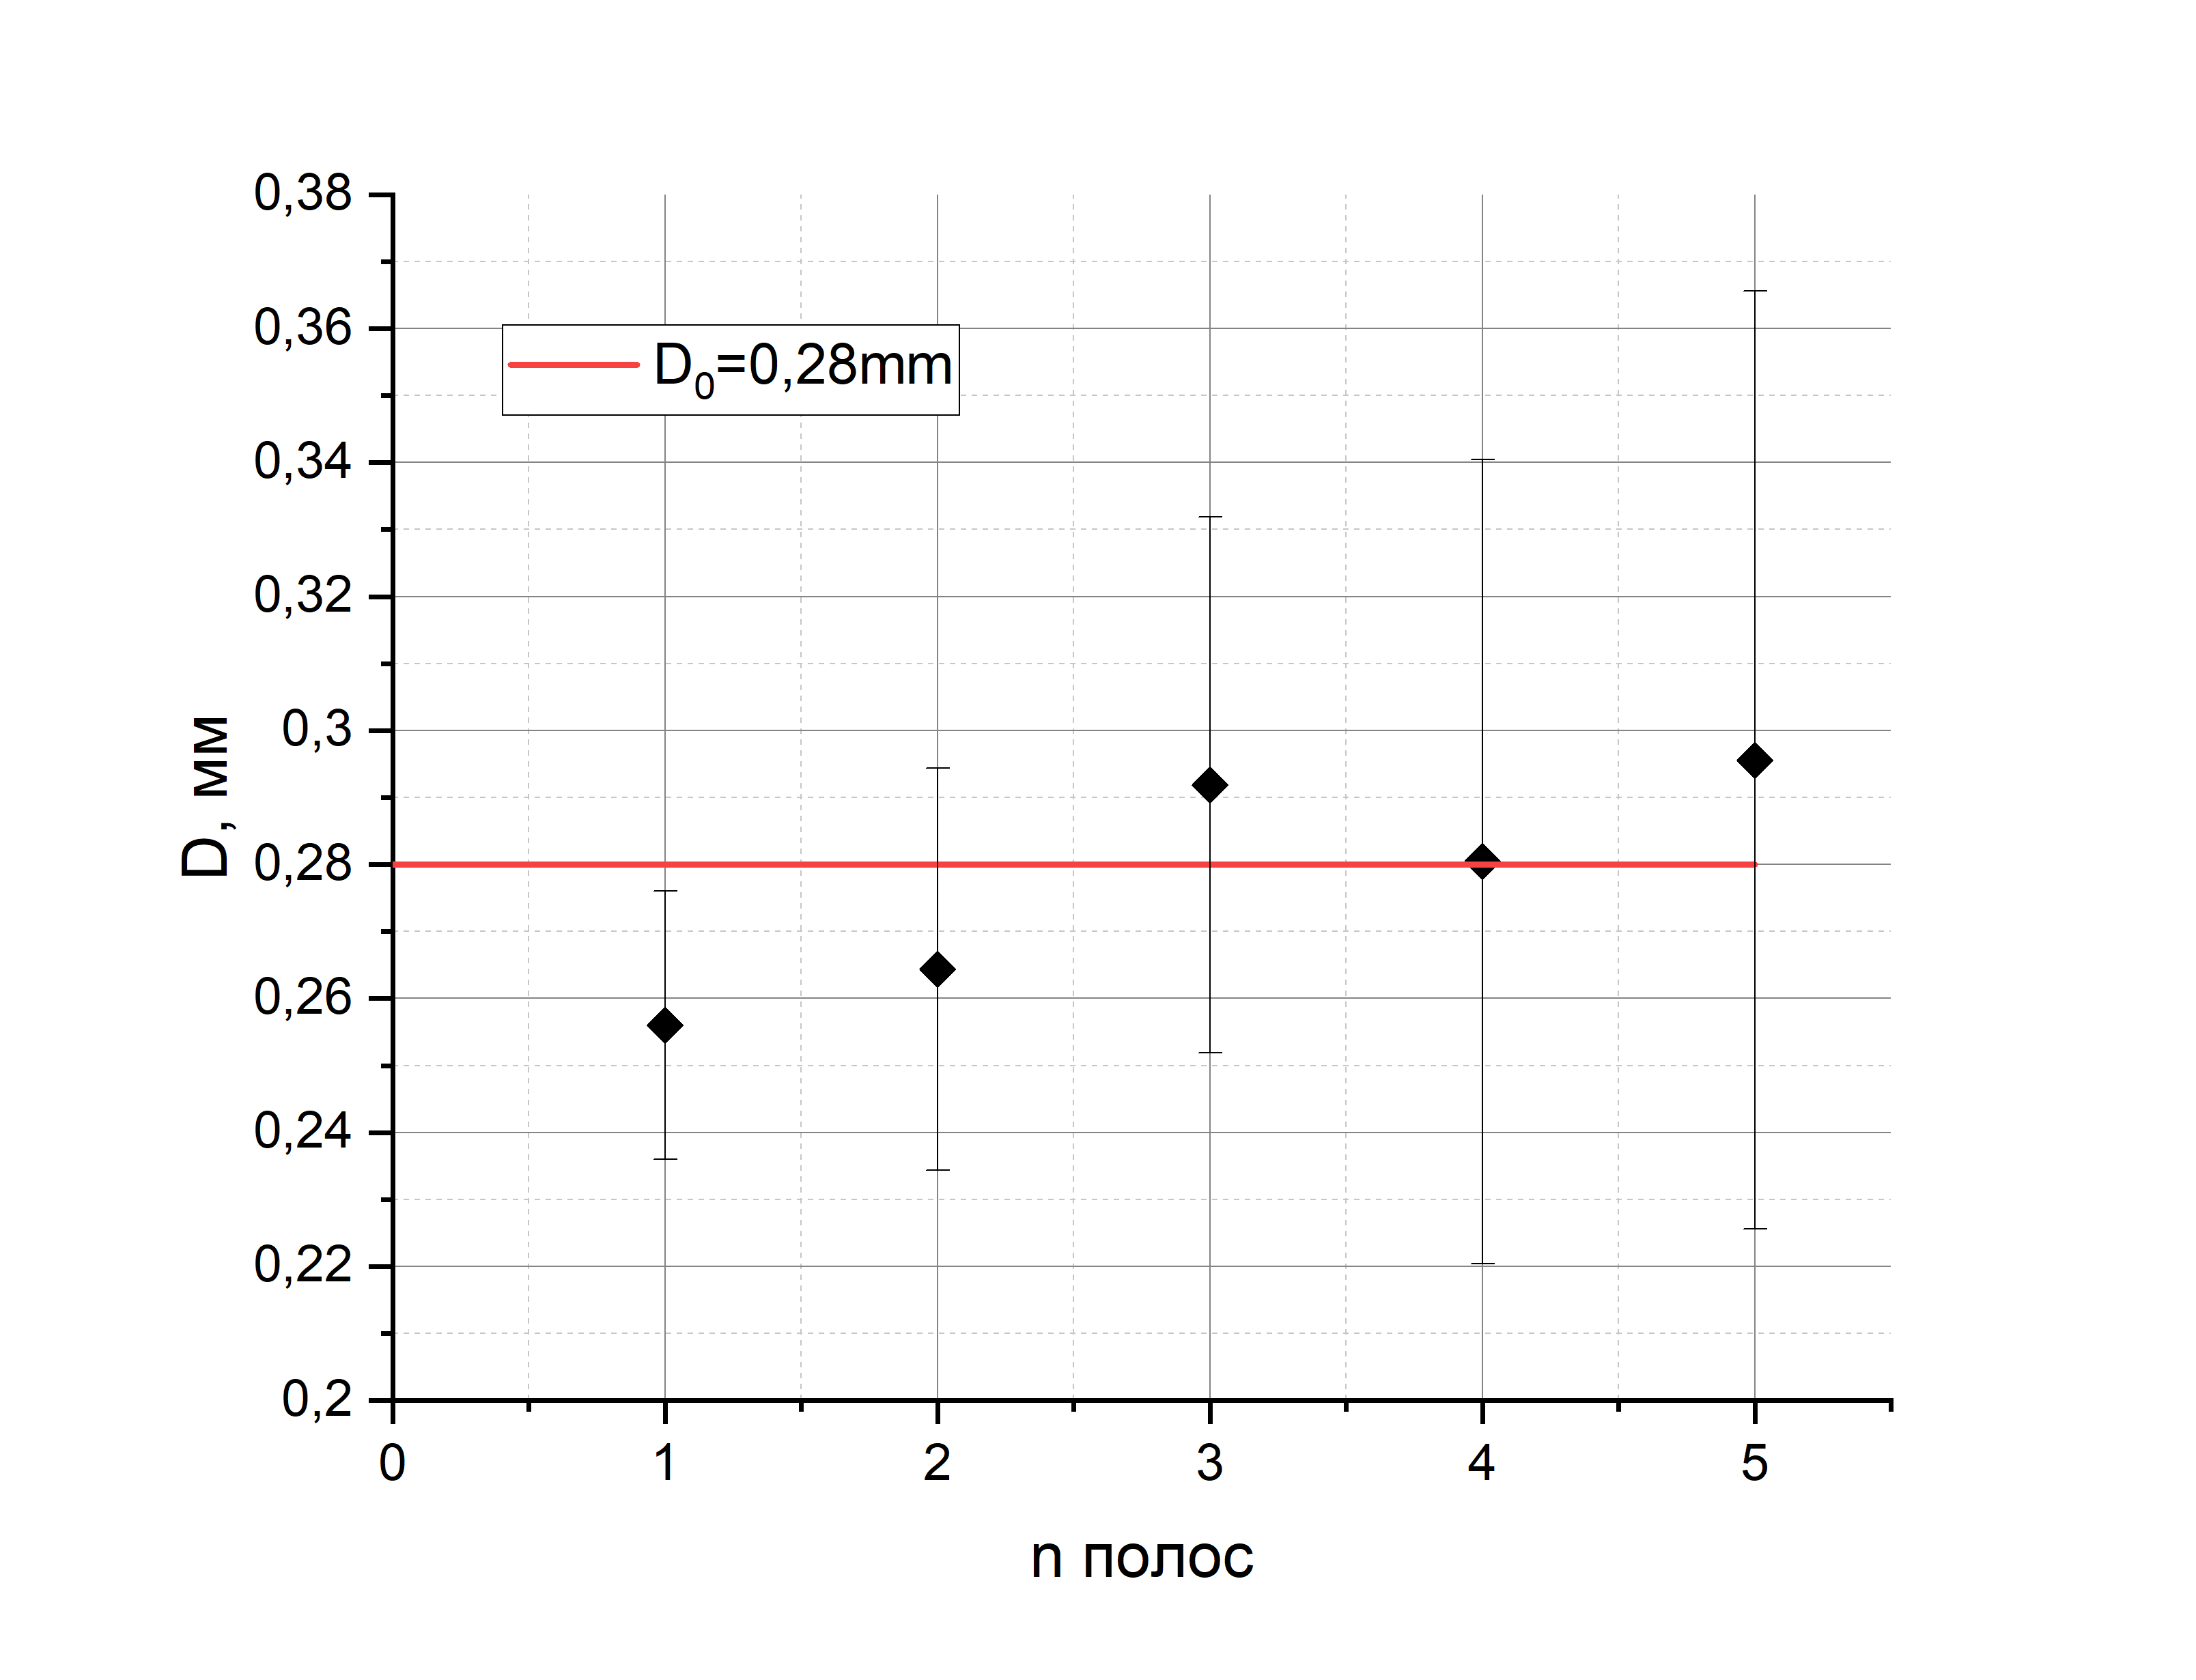
\includegraphics[width=0.8\textwidth]{graph1.png}
    \end{center}
    \caption{D(n)}
\end{figure}
Как видно, расчеты дают сравнительно неплохой результат, хотя погрешность достаточно велика, особенно на большом количестве полос.
%%%%%%%%%%%%%%%%%%%%%%%%%%%%%%%%%%%%%%%%%%%%%%%%%%%%%%%%%%%%%%%%%%%%%%%%%

\newpage

\section{Дифракция Фраунгофера на щели}
	
\subsection{Экспериментальная установка}
На значительном удалении от щели, когда выполнено условие $ C \ll 1 $
(то есть ширина щели становится значительно меньше ширины первой
зоны Френеля, $ b \ll \sqrt{\lambda z} $), изображение щели размывается и возникает
дифракционная картина, называемая дифракцией Фраунгофера.

Дифракцию Френеля и Фраунгофера можно наблюдать на одной
и той же установке (рис. 1). Однако при обычных размерах установки дифракция Фраунгофера возникает только при очень узких щелях.

	\begin{figure}[h!]
		\centering
		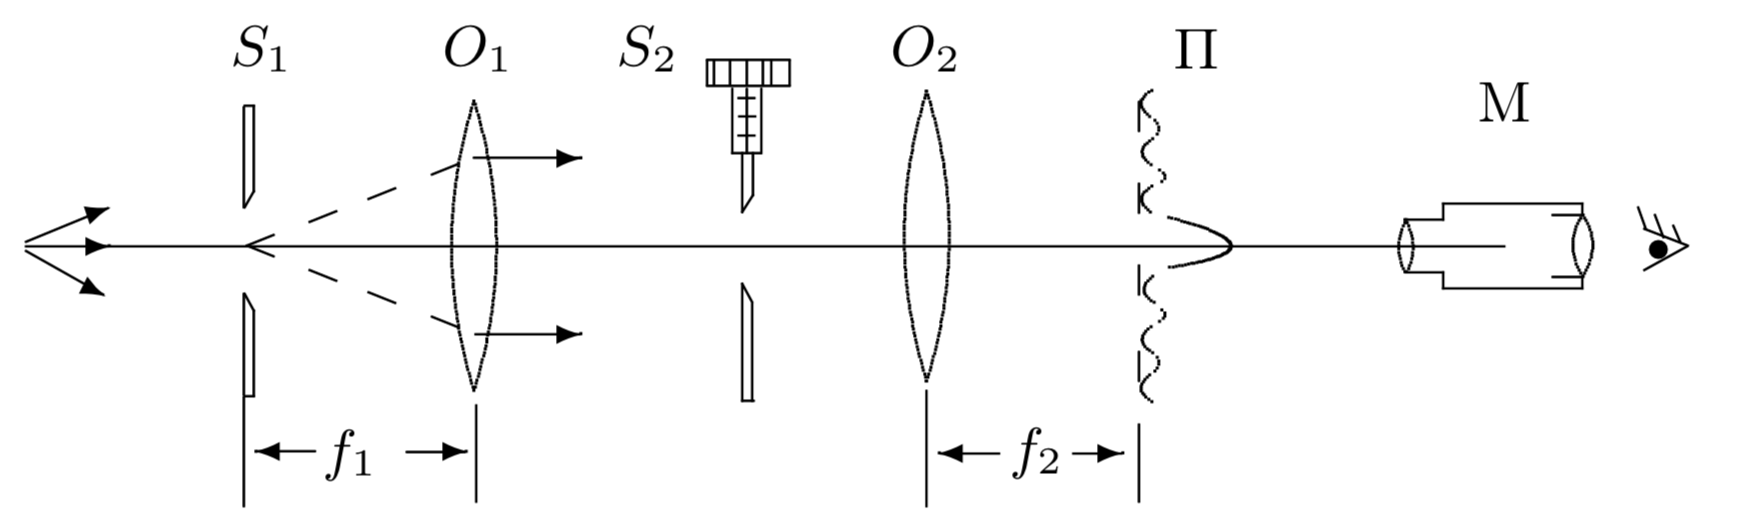
\includegraphics[width=0.8\linewidth]{b.png}
		\caption{Экспериментальная установка B}
		\label{labB}
	\end{figure}

Например, при $ z \approx $ 20-40 см и $  \lambda \approx 5 \x $ 10-5  см получаем$  b \ll 0,3 $ мм. Поскольку работать с такими тонкими щелями неудобно, для наблюдения дифракции Фраунгофера к схеме, изображённой на рис. 1, добавляется объектив $ O_2  $(рис. 3).

Дифракционная картина наблюдается здесь в фокальной плоскости
объектива $ O_2 $. Каждому значению угла $ \theta $ соответствует в этой плоскости точка, отстоящая от оптической оси на расстоянии

\begin{equation}\label{x}
x = f_2 \tg \theta \approx f_2 \theta
\end{equation}

Поскольку объектив не вносит дополнительной разности хода
между интерферирующими лучами (таутохронизм), в его фокальной
плоскости наблюдается неискаженная дифракционная картина Фраунгофера. Эта картина соответствует бесконечно удалённой плоскости
наблюдения.

В центре поля зрения наблюдается дифракционный максимум (светлая полоса). При малых углах $ \theta $ положение минимумов (тёмных полос)
определяется, соотношением

\begin{equation}\label{theta_m}
\theta_m = m \dfrac{\lambda}{b}
\end{equation}

Расстояние $ x_m $ от тёмной полосы до оптической оси объектива $ O_2 $ пропорционально фокусному расстоянию $ f_2 $. Из \eqref{x} и \eqref{theta_m} следует 

\begin{equation}\label{xm}
x_m = m \dfrac{\lambda}{b} f_2
\end{equation}

Видно, что при малых углах минимумы эквидистантны, а
расстояния $ \delta x $ между минимумами обратно пропорциональны ширине $ b $ щели $ S_2 $.

\subsection{Практическая часть}
Координаты $X_m$ для дифракционных полос представлены в таблице 1. Фокусное расстояние объектива $f_2$ = 12.8 см, ширина щели $D_0 = 0.28 \pm 0.1$ мм. По наклону графика (рис. 4) и формуле 4 рассчитаем ширину щели $b = \frac{\lambda f_2}{k} = 281 \pm 5$ мкм, что соответствует ожидаемой.

\begin{table}[h!]
\begin{center}
\caption{Эксперимент с дифракцией Фраунгофера}
\begin{tabular}{|c|c|}
\hline
n  & $X_m$, мм \\ \hline
-5 & 0,8       \\ \hline
-4 & 1         \\ \hline
-3 & 1,24      \\ \hline
-2 & 1,44      \\ \hline
-1 & 1,68      \\ \hline
0  & 2         \\ \hline
1  & 2,32      \\ \hline
2  & 2,54      \\ \hline
3  & 2,76      \\ \hline
4  & 2,98      \\ \hline
5  & 3,2       \\ \hline
\end{tabular}
\end{center}
\end{table}

\begin{figure}[h!]
    \begin{center}
    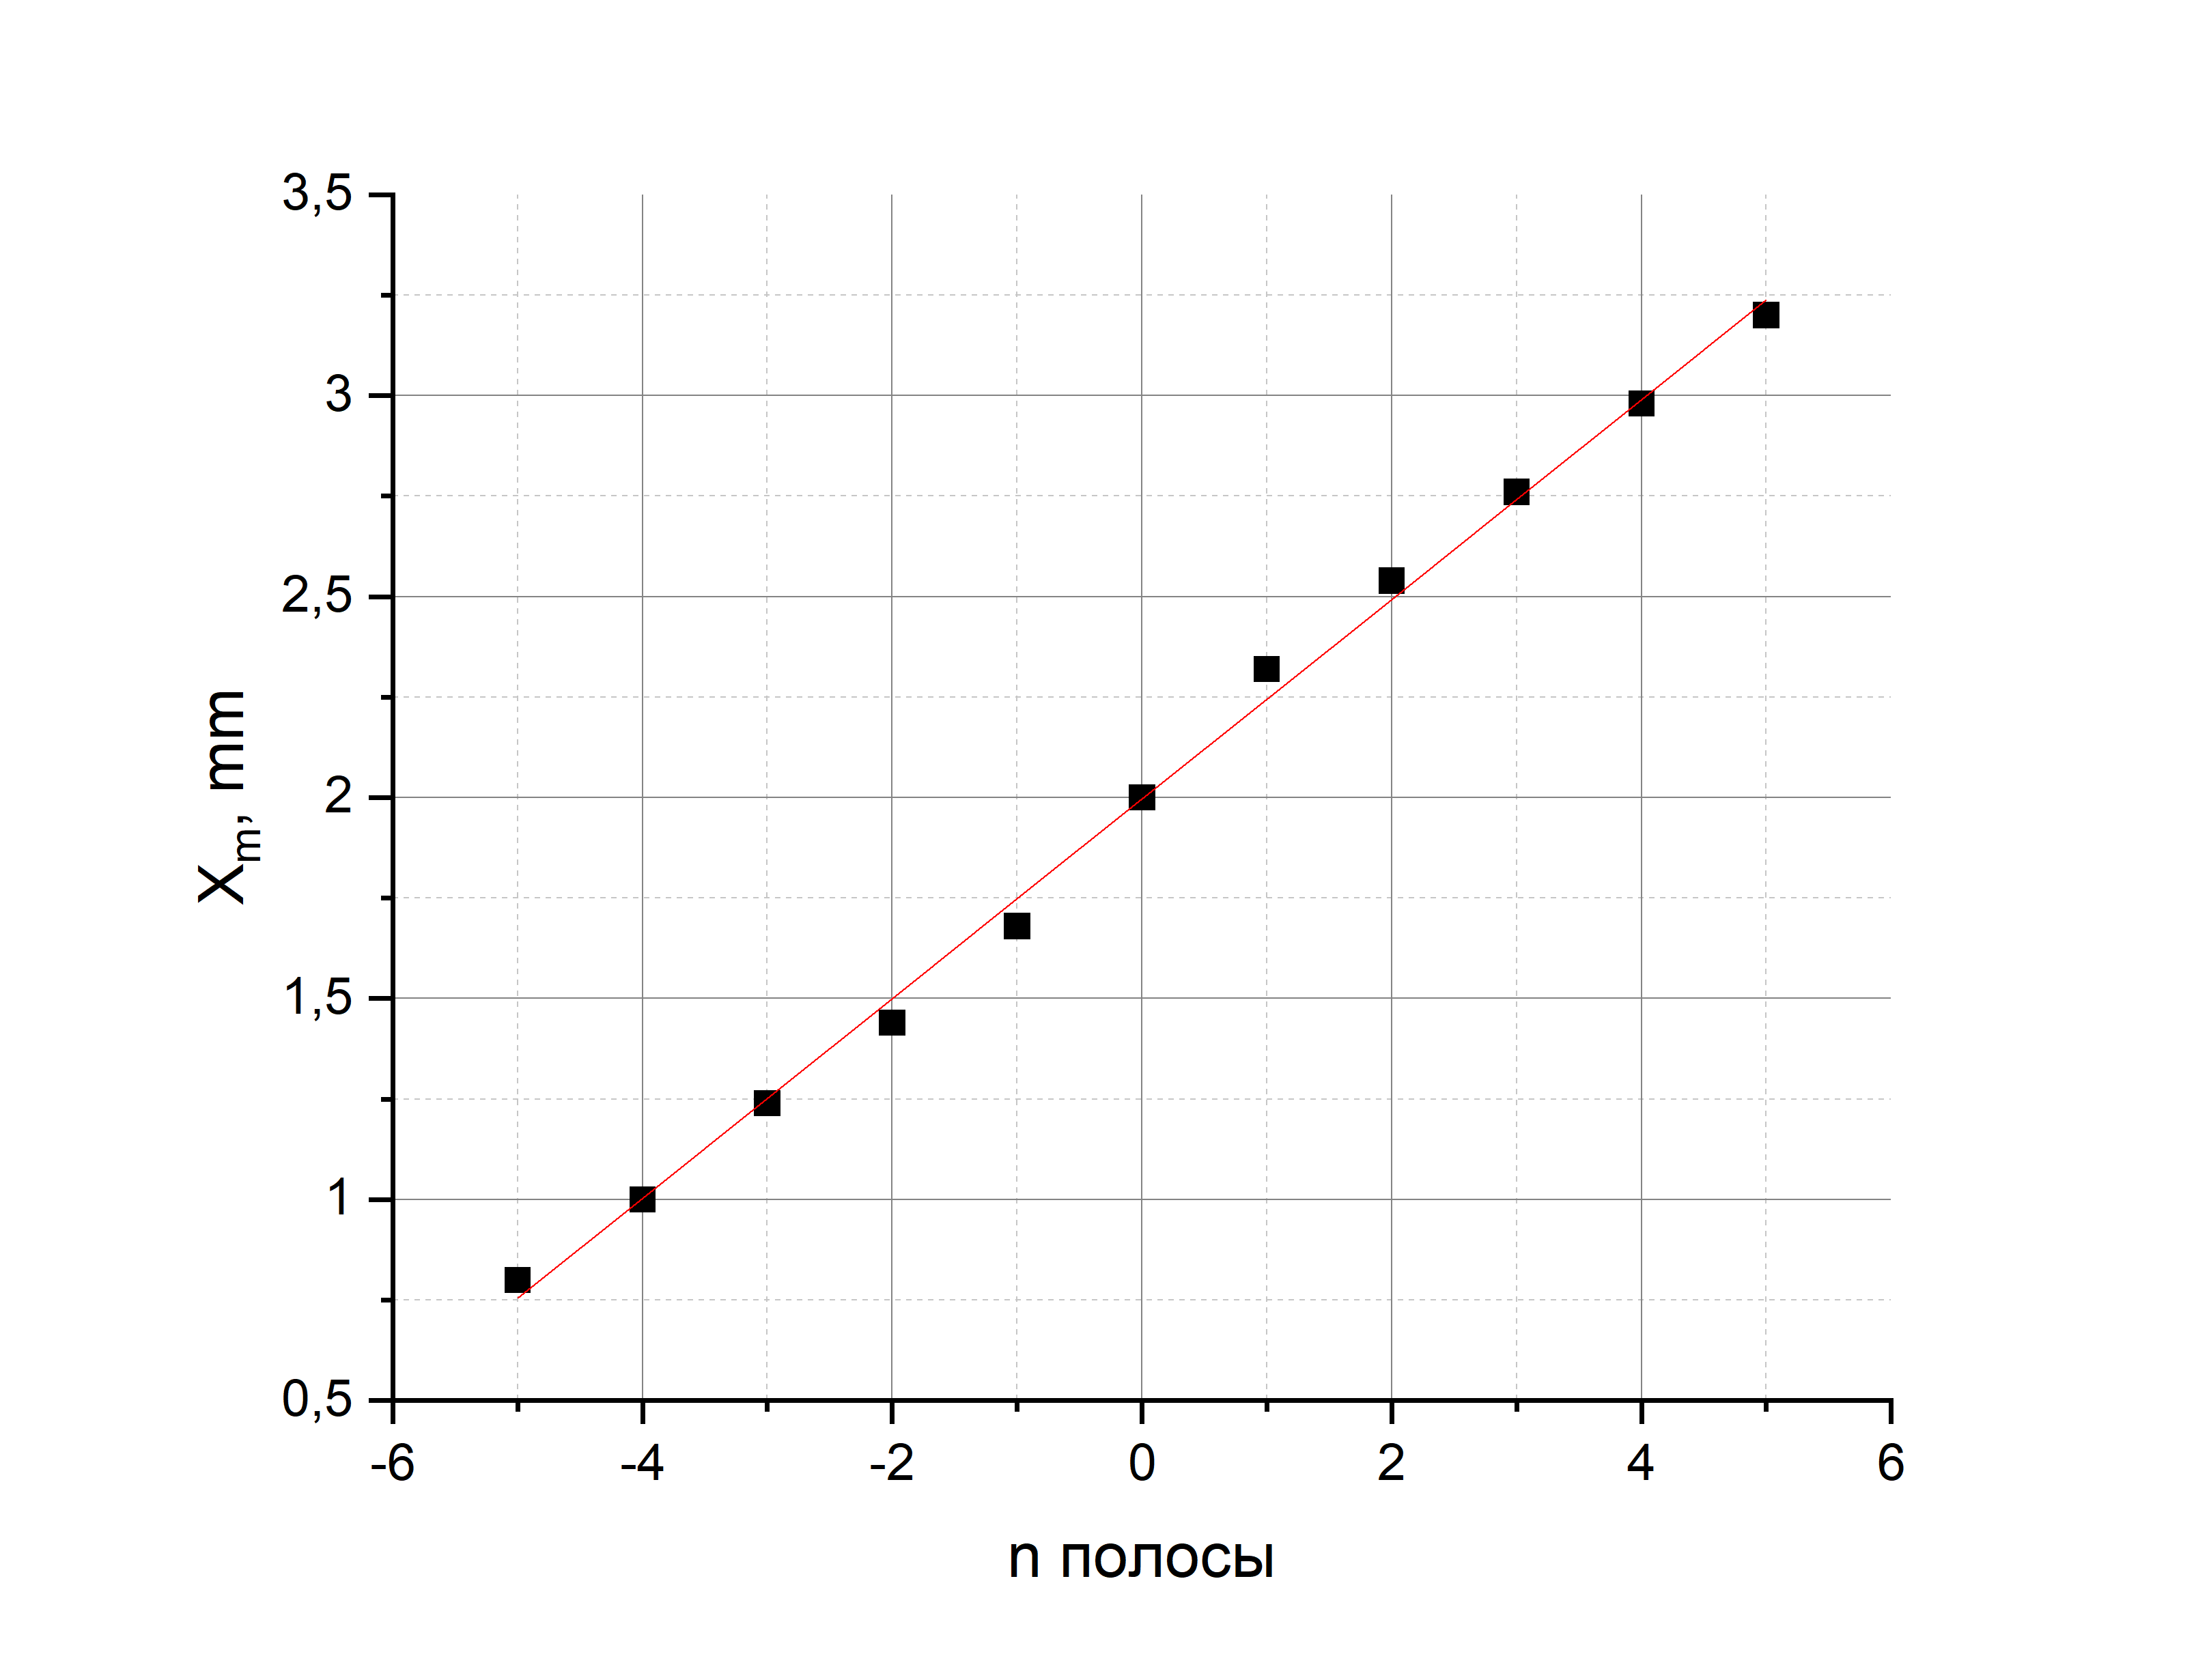
\includegraphics[width=0.8\textwidth]{graph2.png}
    \end{center}
    \caption{$X_m (n)$}
\end{figure}
%%%%%%%%%%%%%%%%%%%%%%%%%%%%%%%%%%%%%%%%%%%%%%%%%%%%%%%%%%%%%%%%%%%%%%%%%

\newpage

\section{Дифракция Фраунгофера на двух щелях}
	
\subsection{Экспериментальная установка}

Для наблюдения дифракции Фраунгофера на двух щелях в установке (рис. 4) следует заменить щель $ S_2 $ экраном Э с двумя щелями
(рис. 6). При этом для оценки влияния ширины входной щели на чёткость дифракционной картины вместо входной щели $ S_1 $ следует поставить щель с микрометрическим винтом. Два дифракционных изображения входной щели, одно из которых образовано лучами, прошедшими через левую, а другое --- через правую щели, накладываются друг на друга.

	\begin{figure}[h!]
		\centering
		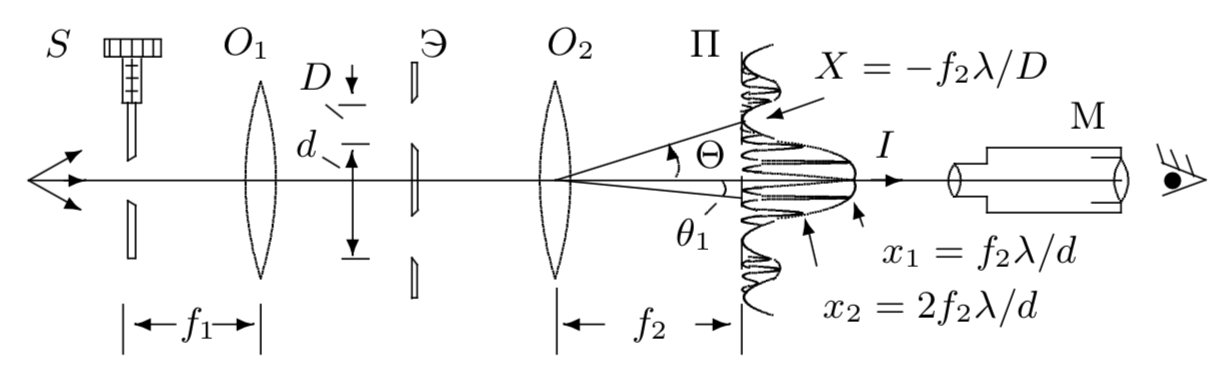
\includegraphics[width=0.8\linewidth]{c.png}
		\caption{Экспериментальная установка C}
		\label{labC}
	\end{figure}

Если входная щель достаточно узка, то дифракционная картина
в плоскости П (рис. 4) подобна той, что получалась при дифракции
на одной щели (рис. 3), однако теперь вся картина испещрена рядом
дополнительных узких полос.
Угловая координата $ \theta_m $ интерференционного максимума $ m $-го порядка определяется соотношением

\begin{equation}\label{}
\theta_m = m \dfrac{\lambda}{b}
\end{equation}

где $ d $ --- расстояние между щелями. Линейное расстояние $ \delta x $ между соседними интерференционными полосами в плоскости П равно, поэтому

\begin{equation}\label{dx}
\delta x = f_2 \dfrac{\lambda}{d}
\end{equation}

На рис. 4 показано распределение интенсивности в фокальной плоскости объектива $ O_2 $. Штриховой линией (в увеличенном масштабе)
изображено распределение интенсивности при дифракции света на одиночной щели. Нетрудно оценить число n интерференционных полос,
укладывающихся в области центрального дифракционного максимума.
Согласно \eqref{xm} полная ширина главного максимума равна $ 2 f_2 \lambda /b $, где $ b $ ширина щели, отсюда

\begin{equation}\label{n}
n = \dfrac{2f_2 \lambda}{b} \dfrac{1}{\delta x} = \dfrac{2d}{b}
\end{equation}

При дифракции света на двух щелях чёткая система интерференционных полос наблюдается только при достаточно узкой ширине входной щели $ S $, которую можно рассматривать как протяжённый источник света размером $ b $. Для наблюдения интерференции необходимо, чтобы расстояние $ d $между щелями не превышало радиуса когерентности

\begin{equation}\label{}
d \ll \dfrac{\lambda}{b} f_1
\end{equation}

Здесь $ b $ --- ширина входной щели $ S $ и, следовательно, $  b/f_1 $ --- её угловая ширина. Таким образом, по размытию интерференционной картины можно оценить размер источника. Этот метод используется в звёздном интерферометре при измерении угловых размеров звёзд.

\subsection{Практическая часть}

Расстояние между соседними интерференционными поллосами $\delta x = \frac{x_1-x_2}{n} = 41.3 \pm 2.5$ мкм, где $x_1, x_2$ - координаты удаленных темных полос, n - число светлых полос между ними. Тогда по формуле (6) можно рассчитать расстояние между щелями $d=f_{2} \frac{\lambda}{\delta x} = 1.7 /pm 0.1$ см. Для сравнения, это же расстояние измеренное с помощью микроскопа $d_0 = 1.81 /pm 0.04$ см, что можно считать достаточно точным совпадением (в пределах погрешности).

Зная ширину главного максимума $h=0,66$ мм, можно расчитать число интерференционных полос внутри этого максимума по формуле (7): $n = \frac{2d}{b} = \frac{dh}{f_2 \lambda} = 16$, что в точности совпадает с наблюдаемым числом полос.
\begin{figure}[h!]
    \begin{center}
    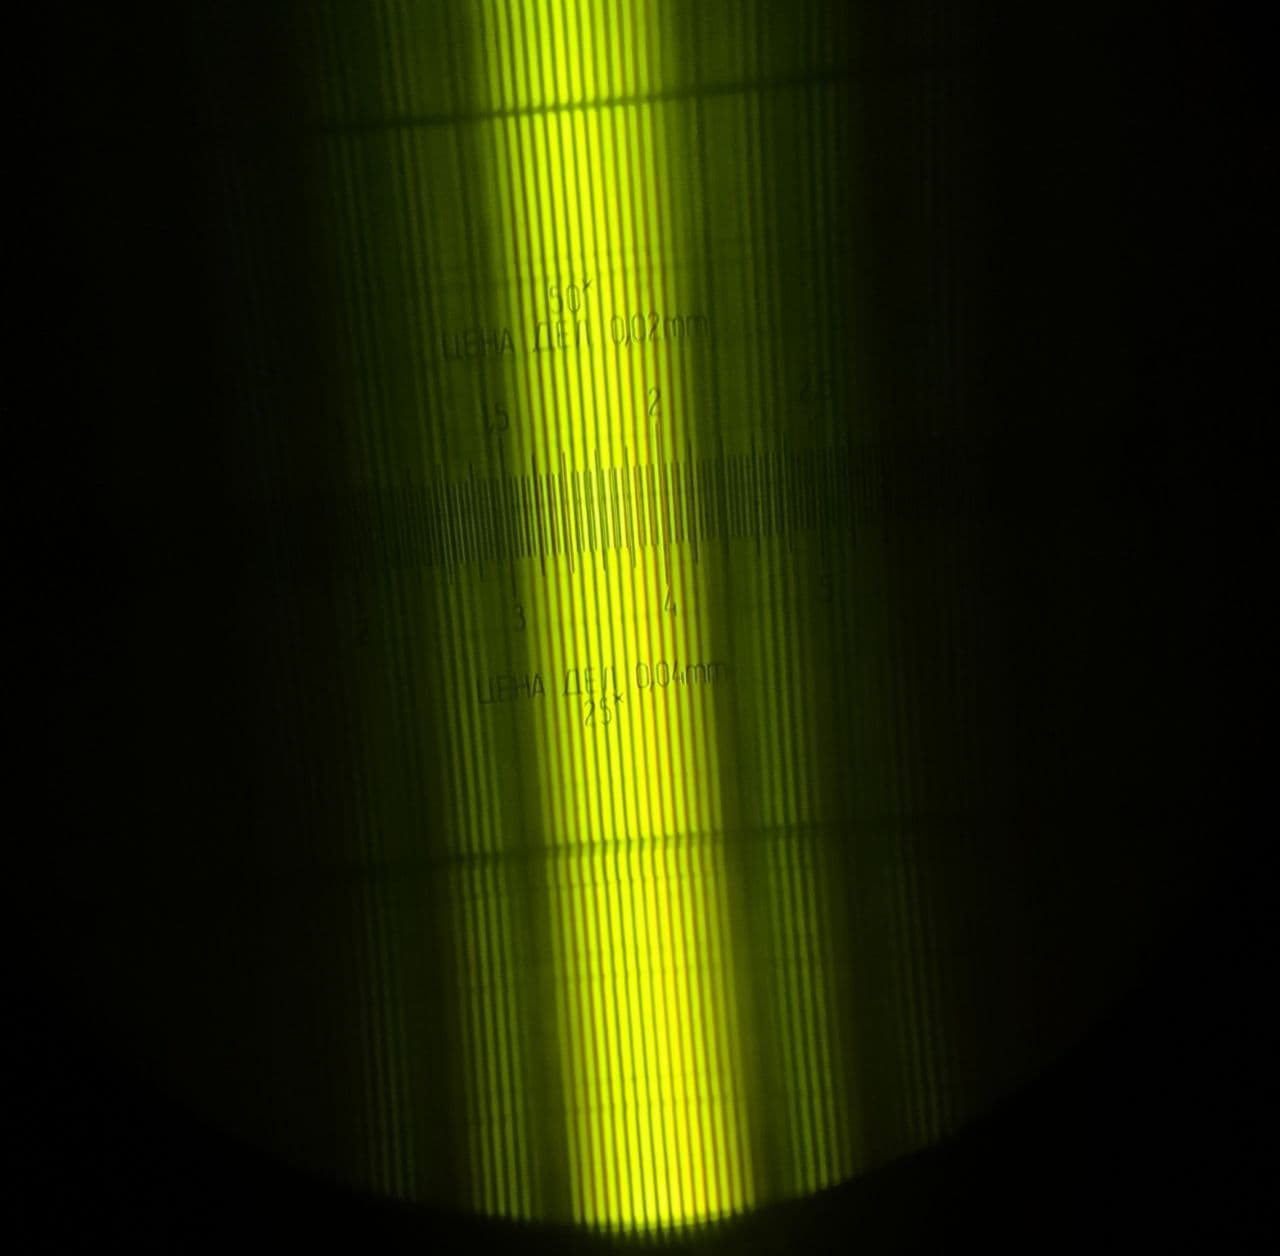
\includegraphics[width=0.8\textwidth]{photo_2021-04-12_16-38-03.jpg}
    \end{center}
    \caption{Дифракционная картина Фраунгофера на 2ух щелях}
\end{figure}

%%%%%%%%%%%%%%%%%%%%%%%%%%%%%%%%%%%%%%%%%%%%%%%%%%%%%%%%%%%%%%%%%%%%%%%%%
 
%%%%%%%%%%%%%%%%%%%%%%%%%%%%%%%%%%%%%%%%%%%%%%%%%%%%%%%%%%%%%%%%%%%%%%%%%
 \section{Выводы}
Были изучены два основных вида дифракции - Френеля и Фраунгофера. Теоретически были рассчитаны различные геометрические параметры установки (ширина щели, расстояние между щелями) и дифракционной картины (количество полос главного максимума). Расчетные величины совпали с измеренными в пределах погрешностей.

\end{document}
